\documentclass[11pt,a4paper]{article}
\usepackage[margin=2.2cm]{geometry}
\usepackage{amsmath,amssymb}
\usepackage{graphicx}
\usepackage{booktabs,multirow,array,tabularx}
\usepackage{xcolor}
\usepackage{xurl}
\usepackage[hidelinks]{hyperref}
\usepackage{enumitem}
\usepackage{caption}
\usepackage{float}
\captionsetup{font=small,labelfont=bf}
\setlist{itemsep=2pt,topsep=4pt}

\newcommand{\nue}{\ensuremath{\nu_e}}
\newcommand{\numu}{\ensuremath{\nu_\mu}}
\newcommand{\code}[1]{\texttt{\small #1}}
\newcommand{\best}[1]{\textbf{#1}}
\newcommand{\pend}{{\color{red!70!black}\scriptsize pending}}
\newcolumntype{L}{>{\raggedright\arraybackslash}X}
\newcommand{\rdone}{332}\newcommand{\rplan}{332}

\makeatletter\newcommand{\tabin}[1]{\@@input #1 }\makeatother

\title{\textbf{Charge + Light Foundation Model for MicroBooNE Open Data:\\ Fairness Controls for the Reference Comparison}\\[4pt]
\large Technical Note --- Round 3}
\author{Haiwang Yu\thanks{Prepared with the assistance of Claude (Anthropic). Code: \url{https://github.com/HaiwangYu/fm4npp-lartpc}, branch \code{main}, package \code{multi-modal-qlmatch/qlfm}. Tracking: GitHub issue \#5. Round~1 (the qlfm model) and round~2 (the comparison with Pandora and four foundation-model recipes) are described in \code{docs/technote-round1.pdf} and \code{docs/technote-round2.pdf}.}}
\date{October 23, 2026}

\begin{document}
\maketitle

\begin{abstract}
\noindent
In round~2, our multi-modal masked autoencoder qlfm-M, which takes TPC charge and PMT light together, was the best model on all four MicroBooNE tasks. A review asked whether that comparison was fair. Four concerns stood out:
\begin{itemize}
  \item the reference models received light only through a weak late-fusion head;
  \item there was no charge-only qlfm at matched size;
  \item qlfm has an extra per-hit embedding for the hit task;
  \item FM4NPP was 4$\times$ smaller and capped at 16{,}384 hits per event.
\end{itemize}

We ran four controls:
\begin{enumerate}
  \item a strong late-fusion head (cross-attention from charge tokens to PMT tokens), identical for every backbone;
  \item a 21M charge-only qlfm (qlfm-M C) with the same pretraining as qlfm-M CL;
  \item a common per-hit adapter for every backbone, plus qlfm without its hit embedding;
  \item FM4NPP without the hit cap, and FM4NPP m4 (19.5M) pretrained for equal node-hours.
\end{enumerate}

Findings:
\begin{itemize}
  \item \textbf{Strong late fusion substantially improves the references,} by up to $+0.21$ hit F1. With it, Panda matches qlfm-M on flavor and energy at 10\% labels.
  \item \textbf{qlfm-M keeps a clear lead at 1\% labels and on the hit task} (0.90 vs 0.79 hit F1).
  \item \textbf{Without light in pretraining, the same 21M qlfm falls behind Panda on every task.} qlfm-M's advantage therefore comes from \emph{fusing light during pretraining}, not from its charge architecture.
  \item \textbf{The hit embedding, FM4NPP's hit cap and its size explain little.}
\end{itemize}

Round~3 used 20.5 Polaris node-hours.
\end{abstract}

\tableofcontents
\clearpage

%=====================================================================
\section{Summary of findings}
%=====================================================================
\begin{enumerate}[leftmargin=*]
\item \textbf{The round-2 late-light baseline understated the references.} An identical, stronger late-fusion head (Sec.~\ref{sec:xf}) raises every reference backbone, most on the per-hit task. Frozen, 1\% labels, hit F1:
  \begin{itemize}
    \item Panda $0.715\to0.792$;
    \item PoLAr-MAE $0.537\to0.712$;
    \item FM4NPP $0.489\to0.700$;
    \item qlfm-S C $0.429\to0.676$.
  \end{itemize}
  Energy improves at 10\% labels, e.g.\ Panda $0.302\to0.272$. Event-level $\nu$ presence changes little (all at 0.96--0.99).

\item \textbf{qlfm-M CL still leads, but the margin depends on the label budget.} Against the best fused reference, Panda + strong fusion:

  \begin{center}\small
  \begin{tabular}{lcc}
  \toprule
   & 1\% labels (qlfm-M vs Panda) & 10\% labels (qlfm-M vs Panda)\\
  \midrule
  T1 hit F1 & \best{0.899} vs 0.792 & \best{0.914} vs 0.823\\
  T3 flavor F1 & \best{0.729} vs 0.706 & 0.764 vs 0.755 (tie)\\
  T4 energy res.\ (lower better) & \best{0.292} vs 0.336 & 0.277 vs \best{0.272} (tie)\\
  T2 event AUC & \best{0.998} vs 0.985 & \best{0.999} vs 0.990\\
  \bottomrule
  \end{tabular}
  \end{center}

  (qlfm-M is quoted with strong fusion too; its own late-light numbers are within $\pm0.02$.) So at 10\% labels, Panda matches qlfm-M on flavor and energy.

\item \textbf{The decisive ingredient is light in pretraining.} qlfm-M C has the same 21M model, tokenizer, objective and 2 node-hours of pretraining as qlfm-M CL, but no light. Frozen at 1\%:

  \begin{center}\small
  \begin{tabular}{lcccc}
  \toprule
   & T2 AUC & T3 F1 & T4 res. & T1 F1\\
  \midrule
  qlfm-M CL & 0.999 & 0.713 & 0.284 & 0.892\\
  qlfm-M C & 0.963 & 0.561 & 0.365 & 0.685\\
  Panda (charge only) & 0.978 & 0.679 & 0.343 & 0.715\\
  \bottomrule
  \end{tabular}
  \end{center}

  qlfm-M C is below Panda on all four tasks. Without any late light, its T2 drops to 0.723 against 0.914 for Panda.
  \begin{itemize}
    \item \textbf{As a charge encoder, Panda is better than our cell-token Transformer.}
    \item \textbf{qlfm-M's round-2 lead comes from pretraining charge and light jointly.}
  \end{itemize}

\item \textbf{qlfm's per-hit embedding does not explain its hit-task lead.} qlfm-M CL scores 0.892 with its own pretrained hit embedding, 0.892 with the common raw adapter, and 0.891 with no per-hit input. A common raw adapter does help the references (Panda $+0.03$, PoLAr-MAE $+0.07$, FM4NPP $+0.06$), but they stay far below 0.89.

\item \textbf{FM4NPP's weak results are not caused by its hit cap or its size.}
  \begin{itemize}
    \item Removing the 16{,}384-hit cap lifts frozen hit F1 from 0.463 to 0.489 (fine-tuned 1\%: $0.620\to0.654$).
    \item Except for a single-seed dip of m3 flavor at 10\% ($0.557\to0.501$), the event tasks are within $\pm0.02$.
    \item The 4$\times$ larger m4 (19.5M) at equal node-hours is at most slightly better than m3.
      \begin{itemize}
        \item Hit F1: $+0.02$ frozen, $+0.03$ fine-tuned (0.685 vs 0.654), $+0.04$ with the raw adapter, $+0.08$ without light.
        \item Flavor at 10\%: 0.571 vs 0.501, where m3's value is the dip above.
        \item Fine-tuned energy is worse (0.409 vs 0.351).
      \end{itemize}
      It stays far below Panda and qlfm-M CL.
  \end{itemize}
\end{enumerate}

%=====================================================================
\section{The fairness questions}
%=====================================================================
Round 2 compared qlfm with the open-data Pandora reconstruction and with four foundation-model recipes: FM4NPP, Panda, PoLAr-MAE and qlfm-SD. All got equal pretraining node-hours, identical heads, label budgets and test sets. Its main limitation is \emph{how light enters each model} (Table~\ref{tab:light}).

\begin{table}[H]\centering\small
\caption{How each model uses PMT light. ``LateLight'' is the round-2 head module; ``strong fusion'' is the round-3 control (Sec.~\ref{sec:xf}).}\label{tab:light}
\begin{tabularx}{\textwidth}{lLL}
\toprule
Model & Light in the pretrained backbone & Light in the downstream head\\
\midrule
qlfm-S/M CL & 32 PMT tokens attend jointly with the charge tokens in every layer; pretrained by masked light reconstruction (40\% of events: all PMTs masked) on 747k events & LateLight (round 2) or strong fusion (round 3)\\
qlfm-S C, qlfm-M C & none & same\\
Panda, PoLAr-MAE, FM4NPP & none (their published recipes are charge-only) & same\\
\bottomrule
\end{tabularx}
\end{table}

The round-2 LateLight head is weak:
\begin{itemize}
  \item \textbf{T2--T4:} the 32 PMT tokens are added to the token set of one attention-pooling layer, so charge and light never interact before pooling.
  \item \textbf{T1:} each hit receives only the event-\emph{mean} light vector.
\end{itemize}
This favours early fusion by construction. The review raised further points:
\begin{itemize}
  \item there was no 21M charge-only qlfm, so fusion and architecture were confounded;
  \item qlfm's hit head receives a pretrained 128-d per-hit embedding;
  \item FM4NPP was run at 4.9M parameters and capped at 16{,}384 hits per event. 47\% of T1 test events exceed the cap, so 9.8\% of the $\nu$ charge got no token and was scored as cosmic.
\end{itemize}

%=====================================================================
\section{Controls}
%=====================================================================
\subsection{Strong late fusion (XFusion)}\label{sec:xf}
XFusion is identical for every backbone:
\begin{enumerate}
  \item Token features are projected to a common 256-d width (LayerNorm + Linear).
  \item Each token cross-attends to the 32 PMT tokens of its event, for 2 layers (8 heads, pre-LN, MLP ratio 2, residual).
  \item The standard heads follow: AttnPool over the fused charge tokens + PMT tokens for T2--T4; for T1, the hit head uses the fused feature of the hit's token plus the mean light.
\end{enumerate}
The PMT tokens come from the same LateLight embedding (per-PMT time profile, PMT position and ID) at 256-d.
\begin{itemize}
  \item \textbf{Size:} about 1.2M trainable parameters for every backbone, 1.15M for 384-d inputs and 1.24M for Panda's 704-d.
  \item \textbf{Training:} from labels only, with the backbone frozen.
  \item \textbf{Runs:} frozen, 1\% and 10\% labels, all four tasks, every backbone.
\end{itemize}

\subsection{qlfm-M C: charge-only qlfm at 21M}
qlfm-M C is identical to qlfm-M CL (384-d, 12 layers, 6 heads, cell tokens, MAE with strip + random masking, 34k steps $\times$ 256 events, 2.0 node-hours) except \code{--light 0}. It is evaluated with the full R2P protocol plus the round-3 controls.

\subsection{Per-hit input for T1}
\begin{itemize}
  \item \textbf{Native:} qlfm passes its pretrained per-hit embedding (in-cell offset, log charge, rms $\to$ 128-d) to the hit head. The other backbones have no such input:
    \begin{itemize}
      \item FM4NPP has one token per hit;
      \item Panda gives each hit its 0.3\,cm voxel feature;
      \item PoLAr-MAE gives a hit only the token of the nearest 4\,cm group.
    \end{itemize}
  \item \textbf{Raw adapter:} the same trainable MLP for every backbone, mapping plane one-hot, normalized wire, tick, log charge and rms to 64-d, replacing the native embedding.
  \item \textbf{None:} qlfm with no per-hit input, so hits in the same cell share a feature.
  \item All frozen at 1\% labels, with round-2 late light.
\end{itemize}

\subsection{FM4NPP: no hit cap, and m4}
\begin{itemize}
  \item \textbf{No cap downstream:} every hit gets a token. Events are micro-batched (8, or 1 when fine-tuning m4), because a forward pass over more than about $10^9$ elements crashes the Mamba2 kernel.
  \item \textbf{m3 uncapped:} the full R2P matrix is re-run.
  \item \textbf{m4:} the paper's ``m4'' size (width 512, $d_\text{state}$ 32, 12 layers, 19.5M parameters), pretrained with the m3 recipe for the same budget: 3.47\,h of training, 36{,}700 steps, 1.17M events, 3.4 node-hours. m3 saw 2.05M events.
\end{itemize}

\subsection{Protocol and compute}
Everything else follows round 2 (R2P):
\begin{itemize}
  \item same splits, label pools and test subsets (10k events; 3k for T1);
  \item 3{,}000-step cap; batch 32;
  \item AdamW, lr $10^{-3}$ frozen and $2\times10^{-4}$ fine-tuned (layer decay 0.9);
  \item best-on-validation checkpoint.
\end{itemize}
Round 3 used 20.5 node-hours (\code{docs/figures/round3\_node\_hours.md}): 5.4 for pretraining (qlfm-M C 2.0, FM4NPP m4 3.4), the rest for 160 downstream runs and a smoke test.

%=====================================================================
\section{Results}
%=====================================================================
\begin{figure}[H]\centering
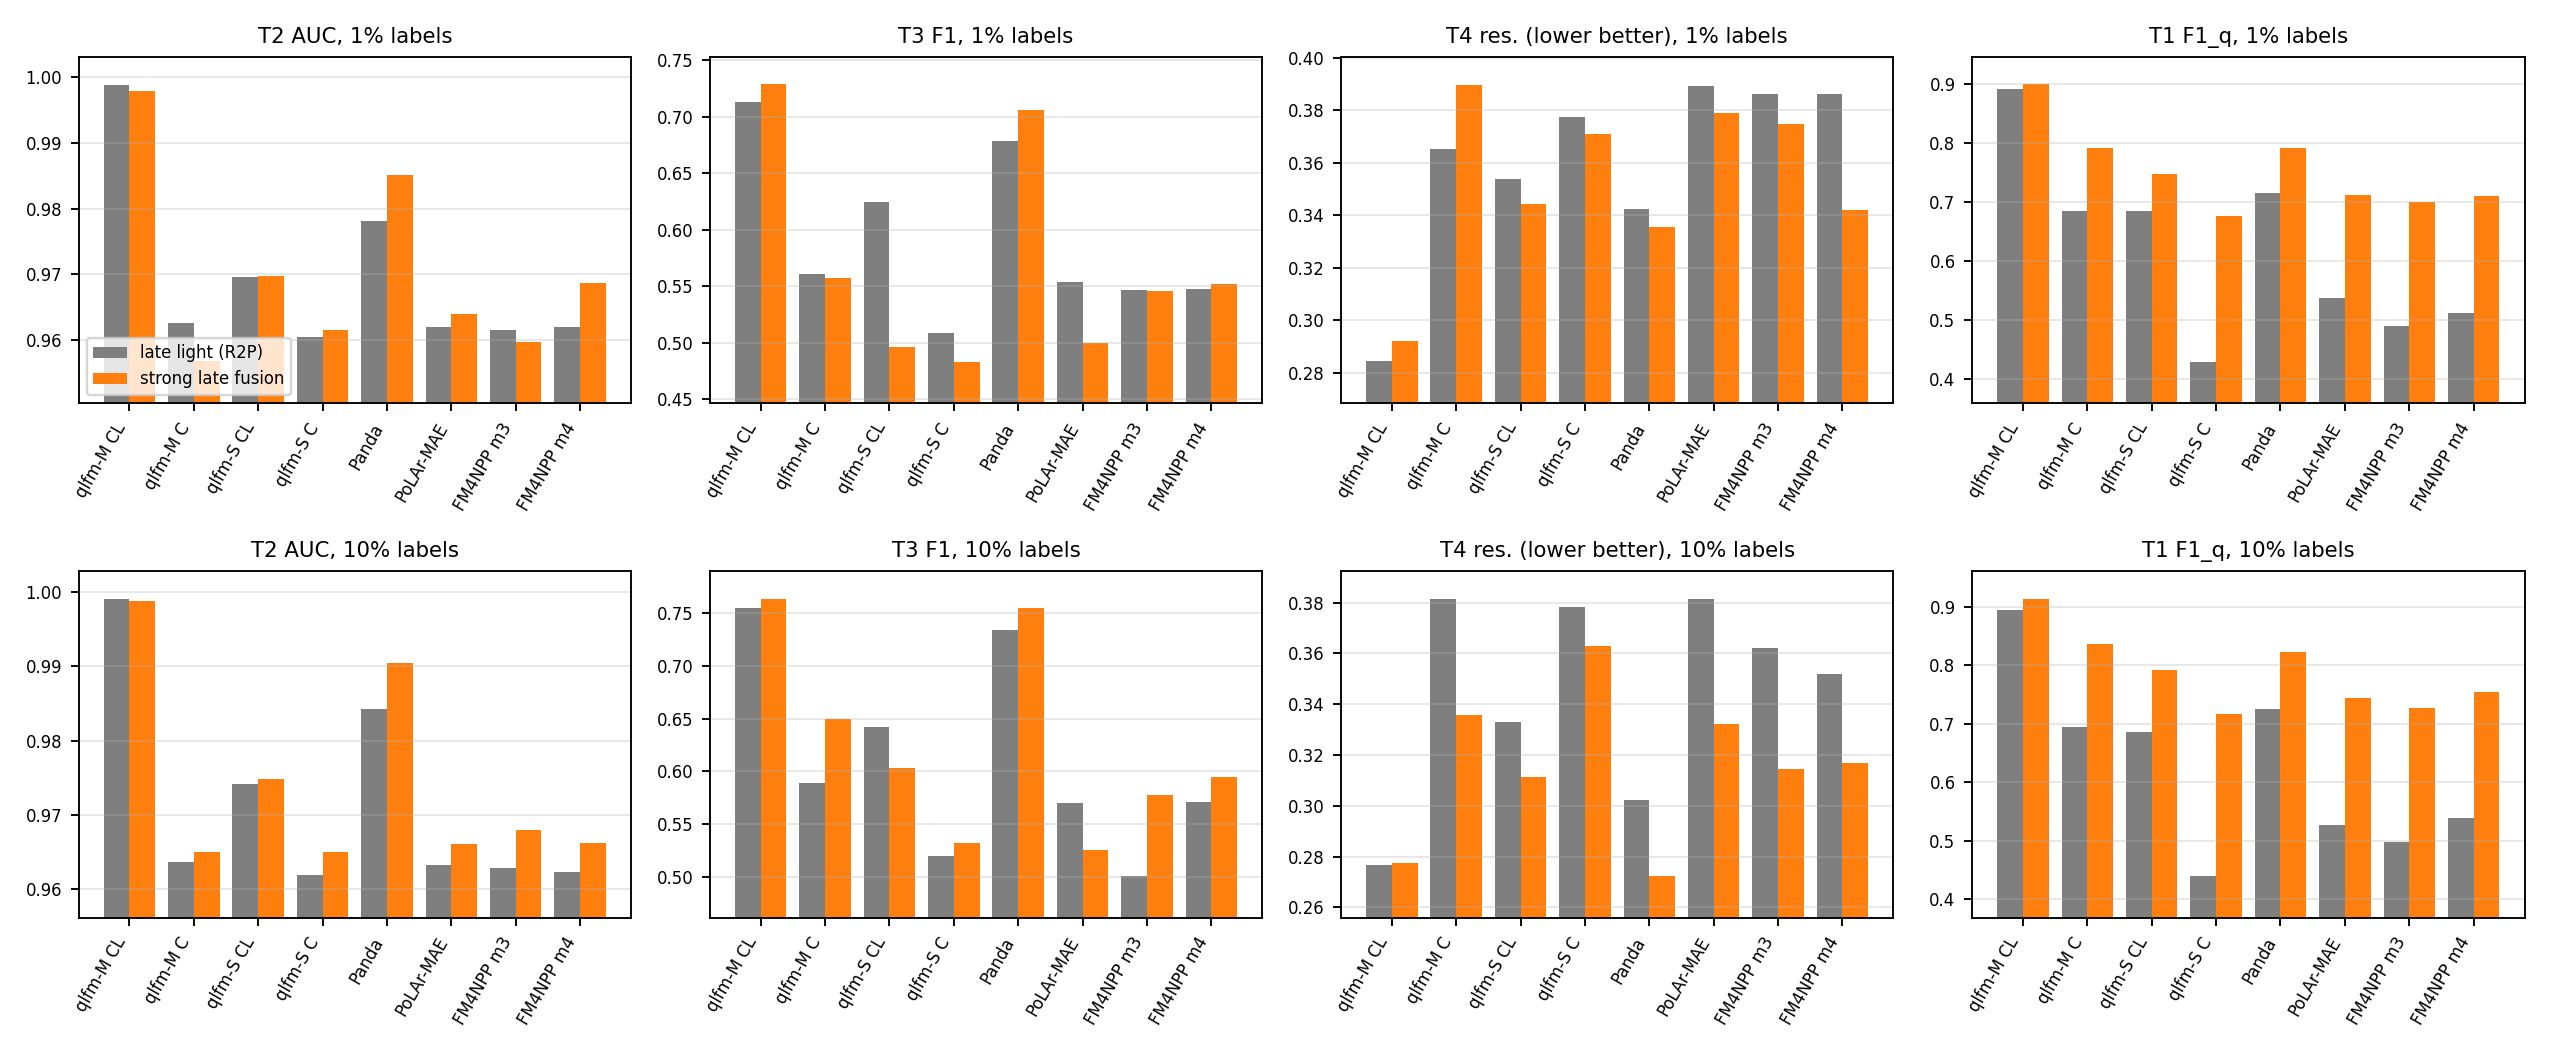
\includegraphics[width=\textwidth]{../figures/round3_fusion.png}
\caption{Frozen backbones with the round-2 late light (grey) and with strong late fusion (orange), at 1\% (top) and 10\% labels (bottom).}\label{fig:xf}
\end{figure}

\newcommand{\xfhead}{\toprule
 & \multicolumn{2}{c}{T2 AUC} & \multicolumn{2}{c}{T3 macro-F1} & \multicolumn{2}{c}{T4 res.\ ($\downarrow$)} & \multicolumn{2}{c}{T1 F1$_q$}\\
Backbone & LL & XF & LL & XF & LL & XF & LL & XF\\\midrule}
\begin{table}[H]\centering\small
\caption{Strong late fusion. Frozen backbone, 1\% labels. LL = round-2 late light, XF = strong late fusion. Best per task in bold. ``FM4NPP m3, capped'' is the round-2 run; all other FM4NPP rows are uncapped.}\label{tab:xf1}
\begin{tabular}{lcccccccc}\xfhead
\tabin{gen/fusion_0.01.tex}
\bottomrule\end{tabular}\end{table}

\begin{table}[H]\centering\small
\caption{As Table~\ref{tab:xf1}, at 10\% labels.}\label{tab:xf10}
\begin{tabular}{lcccccccc}\xfhead
\tabin{gen/fusion_0.1.tex}
\bottomrule\end{tabular}\end{table}

\newcommand{\mxhead}{\toprule
Backbone & frozen 0.1\% & frozen 1\% & frozen 10\% & FT 0.1\% & FT 1\% & no light, 1\%\\\midrule}
\begin{table}[H]\centering\small
\caption{Full R2P matrix for the new backbones (qlfm-M C, FM4NPP m3 uncapped, FM4NPP m4) next to the round-2 rows. ``no light'' is the frozen run without late light; for qlfm-M CL the light inside the backbone remains. $\pm$: spread over 2 seeds.}
\begin{tabular}{lcccccc}\multicolumn{7}{l}{\textbf{T2 event $\nu$/cosmic, AUC}}\\\mxhead
\tabin{gen/matrix_evt_nu.tex}
\bottomrule\end{tabular}

\vspace{6pt}
\begin{tabular}{lcccccc}\multicolumn{7}{l}{\textbf{T3 flavor, macro-F1}}\\\mxhead
\tabin{gen/matrix_flavor.tex}
\bottomrule\end{tabular}
\end{table}

\begin{table}[H]\centering\small
\caption{Full R2P matrix (continued).}
\begin{tabular}{lcccccc}\multicolumn{7}{l}{\textbf{T4 energy, resolution (lower is better)}}\\\mxhead
\tabin{gen/matrix_energy.tex}
\bottomrule\end{tabular}

\vspace{6pt}
\begin{tabular}{lcccccc}\multicolumn{7}{l}{\textbf{T1 hit $\nu$/cosmic, F1$_q$}}\\\mxhead
\tabin{gen/matrix_hit.tex}
\bottomrule\end{tabular}
\end{table}

\begin{table}[H]\centering\small
\caption{T1 per-hit input, frozen at 1\% labels, F1$_q$. Native: the round-2 run, i.e.\ qlfm's pretrained hit embedding, or no per-hit input ($^\ast$) for the other backbones. Raw: common trainable adapter. None: qlfm without a per-hit input. The XF column (strong fusion, native hit input) is shown for reference.}\label{tab:hit}
\begin{tabular}{lcccc}\toprule
Backbone & native & raw adapter & none & XF (native)\\\midrule
\tabin{gen/hitfeat.tex}
\bottomrule\end{tabular}\end{table}

%=====================================================================
\section{Discussion}
%=====================================================================
\paragraph{Was round 2 fair?}
In protocol yes (same data, labels, heads, budgets), in light handling no: the references could use light only through a head that cannot match charge with light.
\begin{itemize}
  \item Once that head is strengthened, the references gain a lot, and at 10\% labels Panda is on par with qlfm-M on flavor and energy.
  \item The round-2 statement ``qlfm-M is best on all four tasks from 1\% labels'' still holds for 1\% labels and for the hit task, but not uniformly at 10\%.
\end{itemize}

\paragraph{Why early fusion wins where it does.}
$\nu$/cosmic separation is largely a charge--light \emph{matching} problem: which charge is in time and in position with the beam flash.
\begin{itemize}
  \item With light inside the backbone, MAE pretraining forces the charge tokens to predict the PMT pattern. This learns the matching from 747k unlabelled events.
  \item A head must instead learn it from 300--7{,}000 labelled events. Strong late fusion closes much of the gap when labels are plentiful (10\%), but not with 1\% labels or for per-hit decisions.
  \item This also explains why qlfm-M CL itself barely changes with strong fusion: its tokens already carry the matched light.
\end{itemize}

\paragraph{Which charge encoder is better.}
At matched size and compute, Panda (PTv3 + Sonata self-distillation) is a better charge-only encoder than qlfm's cell-token MAE. This holds with the R2P head (better on all four tasks), with strong late fusion (T2--T4 clearly better; T1 equal at 1\% and 0.823 vs 0.837 at 10\%), and without any light (T2 0.914 vs 0.723). FM4NPP m3, FM4NPP m4 and qlfm-M C form a second group at about the same level. A natural next step is to combine the two strengths: Panda-style charge encoding with light fused during pretraining.

\paragraph{Smaller effects.}
\begin{itemize}
  \item \textbf{Hit embedding:} qlfm's hit embedding is irrelevant at 21M (0.892 / 0.892 / 0.891) and matters only for the small charge-only model. A per-hit raw adapter is a cheap, general improvement for the point-cloud references (PoLAr-MAE $+0.07$, FM4NPP m3/m4 $+0.06$/$+0.07$).
  \item \textbf{FM4NPP cap:} removing it is worth $\approx$0.03 hit F1.
  \item \textbf{FM4NPP size:} at equal node-hours, 4$\times$ more parameters (m4, 1.17M events) gives at most small gains over m3 (2.05M events).
  \item \textbf{Strong fusion at 1\% labels on flavor:} it sometimes overfits, e.g.\ qlfm-S CL $0.624\to0.496$ and PoLAr-MAE $0.554\to0.500$. The extra 1.2M head parameters are large for about 3k labelled events.
\end{itemize}

%=====================================================================
\section{Limitations}
%=====================================================================
\begin{itemize}[leftmargin=*]
\item Single seed except frozen 0.1\%; differences below about 0.02 are not significant.
\item Strong fusion was run frozen only. Fine-tuning with it, and combining it with the raw hit adapter, are not tested.
\item The references remain charge-only in pretraining. Giving them light during pretraining (the fair ``early fusion for everyone'' test) needs changes to each recipe and is left open.
\item Home advantage remains: qlfm's design was iterated on this dataset in round~1; the references use one untuned adaptation each.
\item The FM4NPP m4 fine-tune runs first ran out of memory at micro-batch 4. They were re-run at micro-batch 1 (same batch of 32 events); the 1\% runs needed one save/resume across jobs and all reached their full step count.
\end{itemize}

%=====================================================================
\section{Reproducibility}
%=====================================================================
\sloppy
\begin{itemize}[leftmargin=*]
\item Code (commit on \code{main}):
  \begin{itemize}
    \item \code{qlfm/models/heads.py}: \code{XFusion}, \code{RawHit};
    \item \code{qlfm/train\_downstream.py}: \code{--late-light 2}, \code{--hit-feat}, \code{--max-hits}, \code{--resume};
    \item \code{qlfm/ref/fm4npp.py}: cap override.
  \end{itemize}
\item Tasks: \code{scripts/make\_tasks\_r3.py OUT \{xf,hit,r2p\} BACKBONE...}, run by \code{scripts/run\_queue.sh}.
\item Pretraining:
  \begin{itemize}
    \item qlfm-M C: \code{qlfm.train\_pretrain --light 0 --d 384 --depth 12 --heads 6 --steps 34000 --bs 64}.
    \item FM4NPP m4: \code{--method fm4npp --d 512 --d-state 32 --budget-h 3.47} (mamba venv).
  \end{itemize}
\item Tables and figure: \code{scripts/summarize\_r3.py R2P\_ROOT R3\_ROOT docs/technote-round3-tex/gen docs/figures/round3\_fusion.png}. Unfinished runs print as \pend, so the note is rebuilt by re-running it.
\end{itemize}

\end{document}
